\documentclass{article}
\usepackage{graphicx} % Required for inserting images
\usepackage[left=2cm,right=2cm,top=2.5cm,bottom=2.5cm]{geometry}
\usepackage[catalan]{babel}
\usepackage{pdfpages}
\usepackage{algorithm}
\usepackage{algorithmic}
\usepackage{minted}
\usepackage{caption}
\usepackage{array}   
\usepackage{graphicx}
\usepackage{float}
\graphicspath { {images/} }
\usepackage{hyperref}
\usepackage{tikz}
\usepackage{amsmath}
\usepackage{bm}
\usepackage{amssymb}
\usepackage{listings}
\usepackage{xcolor}
\usepackage{amssymb}
\floatname{algorithm}{Algorisme}

\begin{document}

\begin{titlepage}
    \centering
    {\bfseries\large Universitat de les Illes Balears \par 
    \vspace{1cm}}
    {\scshape\Huge Cerques \par}
    \vspace{1cm}
    {\itshape\Large Intel·ligència Artificial \par}
    \vfill
    {\Large Marc Ferrer i Harpo Joan\par}
\vfill
{\Large Febrer 2025 \par}
\vfill
\end{titlepage}

\newpage

\tableofcontents

\newpage

\section{Introducció i descripció del problema}
El camp de la intel·ligència artificial inclou diverses tècniques algorísmiques fonamentals, entre les quals hi trobem les cerques. Aquesta tècnica és una eina molt útil per resoldre problemes i optimitzar la recerca de solucions. Per aquest motiu, és àmpliament utilitzada en diferents contextos dins de la intel·ligència artificial. En aquest projecte, aplicarem diversos algorismes de cerca de diferents tipologies per comparar els resultats obtinguts. Tot i que totes aquestes estratègies de resolució arriben a una solució correcta, l’aspecte més interessant és analitzar l’eficiència amb què s'aconsegueix, tenint en compte el temps i els recursos computacionals utilitzats, que esdevenen cada cop més fonamentals en un món digitalment industrialitzat.

\section{Els algorismes de cerca}
Segons aquest \href{https://www.geeksforgeeks.org/search-algorithms-in-ai/}{blog} sobre IA, els problemes resolubles amb tècniques de cerca presenten fonamentalment un estat inicial i un de final, inclosos dins un \textbf{conjunt d'estats}. Per trobar-ne l'estat final partint del primer, s'ha de trobar un \textbf{camí}, el qual és generat per un algorisme de cerca. Llavors, si recordam l'idea d'\href{https://en.wikipedia.org/wiki/Intelligent_agent}{\textit{agent intel·ligent}} i aplicam aquest concepte de cerca, podem imaginar la solució a un problema com una espècie d'\textit{explorador} dins el nostre particular univers (que és el conjunt d'estats).

Com tots els exploradors, n'hi ha que en saben les rutes i n'hi ha que no. En el context que ens referim, es poden distingir entre els \textit{Uninformed-Search algorithms} i els \textit{Informed-Search algorithms}. Aquestes estratègies es diferencien en que els primers no tenen informació addicional de la solució a mesura que es realitza la cerca; també es conneix com \textit{Blind-Search} i en aquest \href{https://www.cs.ucdavis.edu/~vemuri/classes/ecs170/blindsearches_files/blind_searches.htm}{exemple} se'n poden observar alguns dels desavantatges que presenta. D'altra banda, els algorismes informats presenten algún tipus de tècnica que els hi proveeix informació sobre si s'apropen o allunyen de la solució. És per això que, en general, són més eficients i amb el desenvolupament d'aquesta pràctica ho demostrarem.

\subsection{\textit{Depth-First Uninformed Search}}
Els algorismes no-informats són el cas més ineficient del que parlarem. Se'n poden distingir diverses estratègies de cerca no informada: \textit{breadth-first}, \textit{iterative deepening search}, \textit{depth-limited} o \textit{depth-first}. Tots aquests són similars però la cerca que realitzen prioritza certes característiques que, depenent del problema, són més adients en cada cas. En la següent figura es pot observar com l'elecció de l'estratègia determina la forma en que s'arriba a una solució. 

\begin{figure}[h]
    \centering
    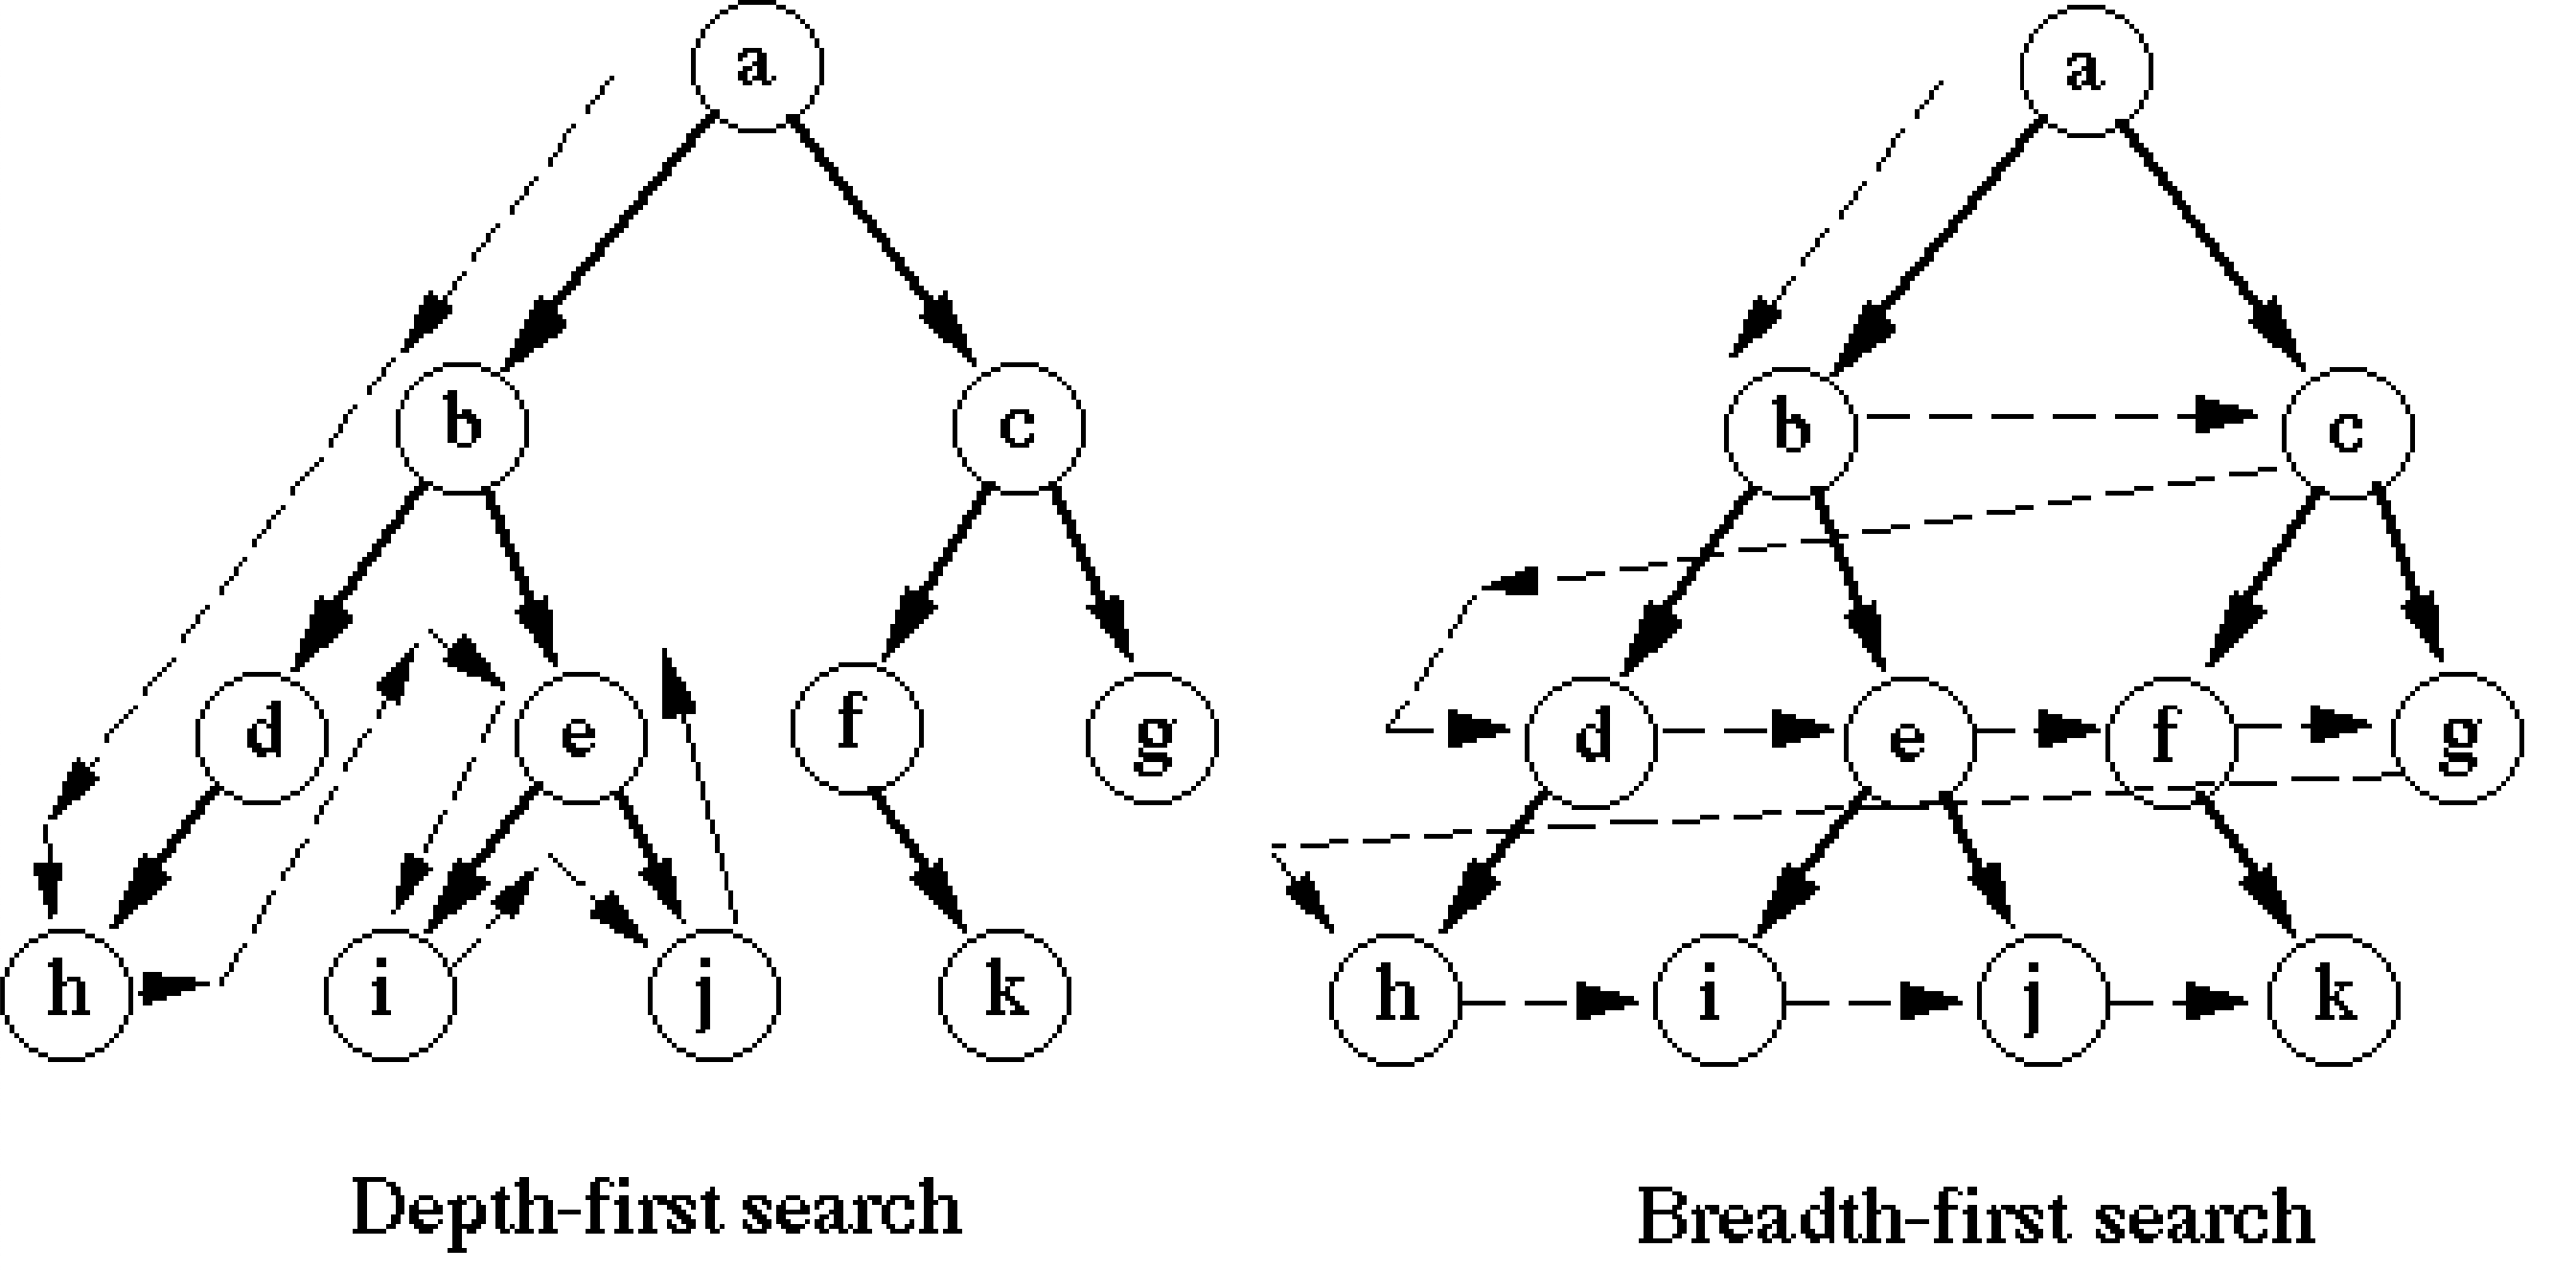
\includegraphics[width=0.8\textwidth]{tree}
    \caption{Arbres generats pels algorismes de cerca}
    \label{fig:Tree}
\end{figure}

\subsubsection{Codi desenvolupat}
El desenvolupament de l'algorisme de cerca profunda per al nostre agent l'hem fet partint de la base exposada al \href{https://github.com/miquelmn/ia_2024/tree/master}{repositori de l'assignatura}. Conceptualment, aquest algorisme comprova que l'estat en que ens trobam hagi estat visitat o si n'és la solució mentre hi hagi estats disponibles. Com podem veure, es tracta d'un algorisme simple


\begin{minted}{python}
def cerca(self, estat_inicial: Estat) -> bool:

    self.__oberts = [estat_inicial]
    self.__tancats = set()
    trobat = False
    actual = None

    while self.__oberts:
        actual = self.__oberts.pop(-1)
        if actual in self.__tancats:
            continue
        if actual.es_meta():
            self.__accions = actual.accions
            trobat = True
            break
        for f in actual.genera_fills():
            self.__oberts.append(f)
        self.__tancats.add(actual)

    return trobat
\end{minted}

\subsubsection{Primers resultats}

Aplicar la priorització del desplegament dels nodes amb profunditat fa que l'arbre de desició generat sigui molt ineficient. Per a obtenir unes dades suficientment riguroses i poder comparar \textit{a posteriori} quin és el rendiment de l'algorisme comparat amb els altres, s'han obtingut mètriques temporals fent ús de la llibreria \verb|time| indicades a la \autoref{sec:conclusions}. A més, s'ha fet ús de l'eina \verb|Profiling|, la qual ens demostra que aquest mètode abusa dels recursos computacionals amb fins a \textbf{38088 cridades} a la funció \verb|deepcopy|. 

\begin{figure}[h]
    \centering
    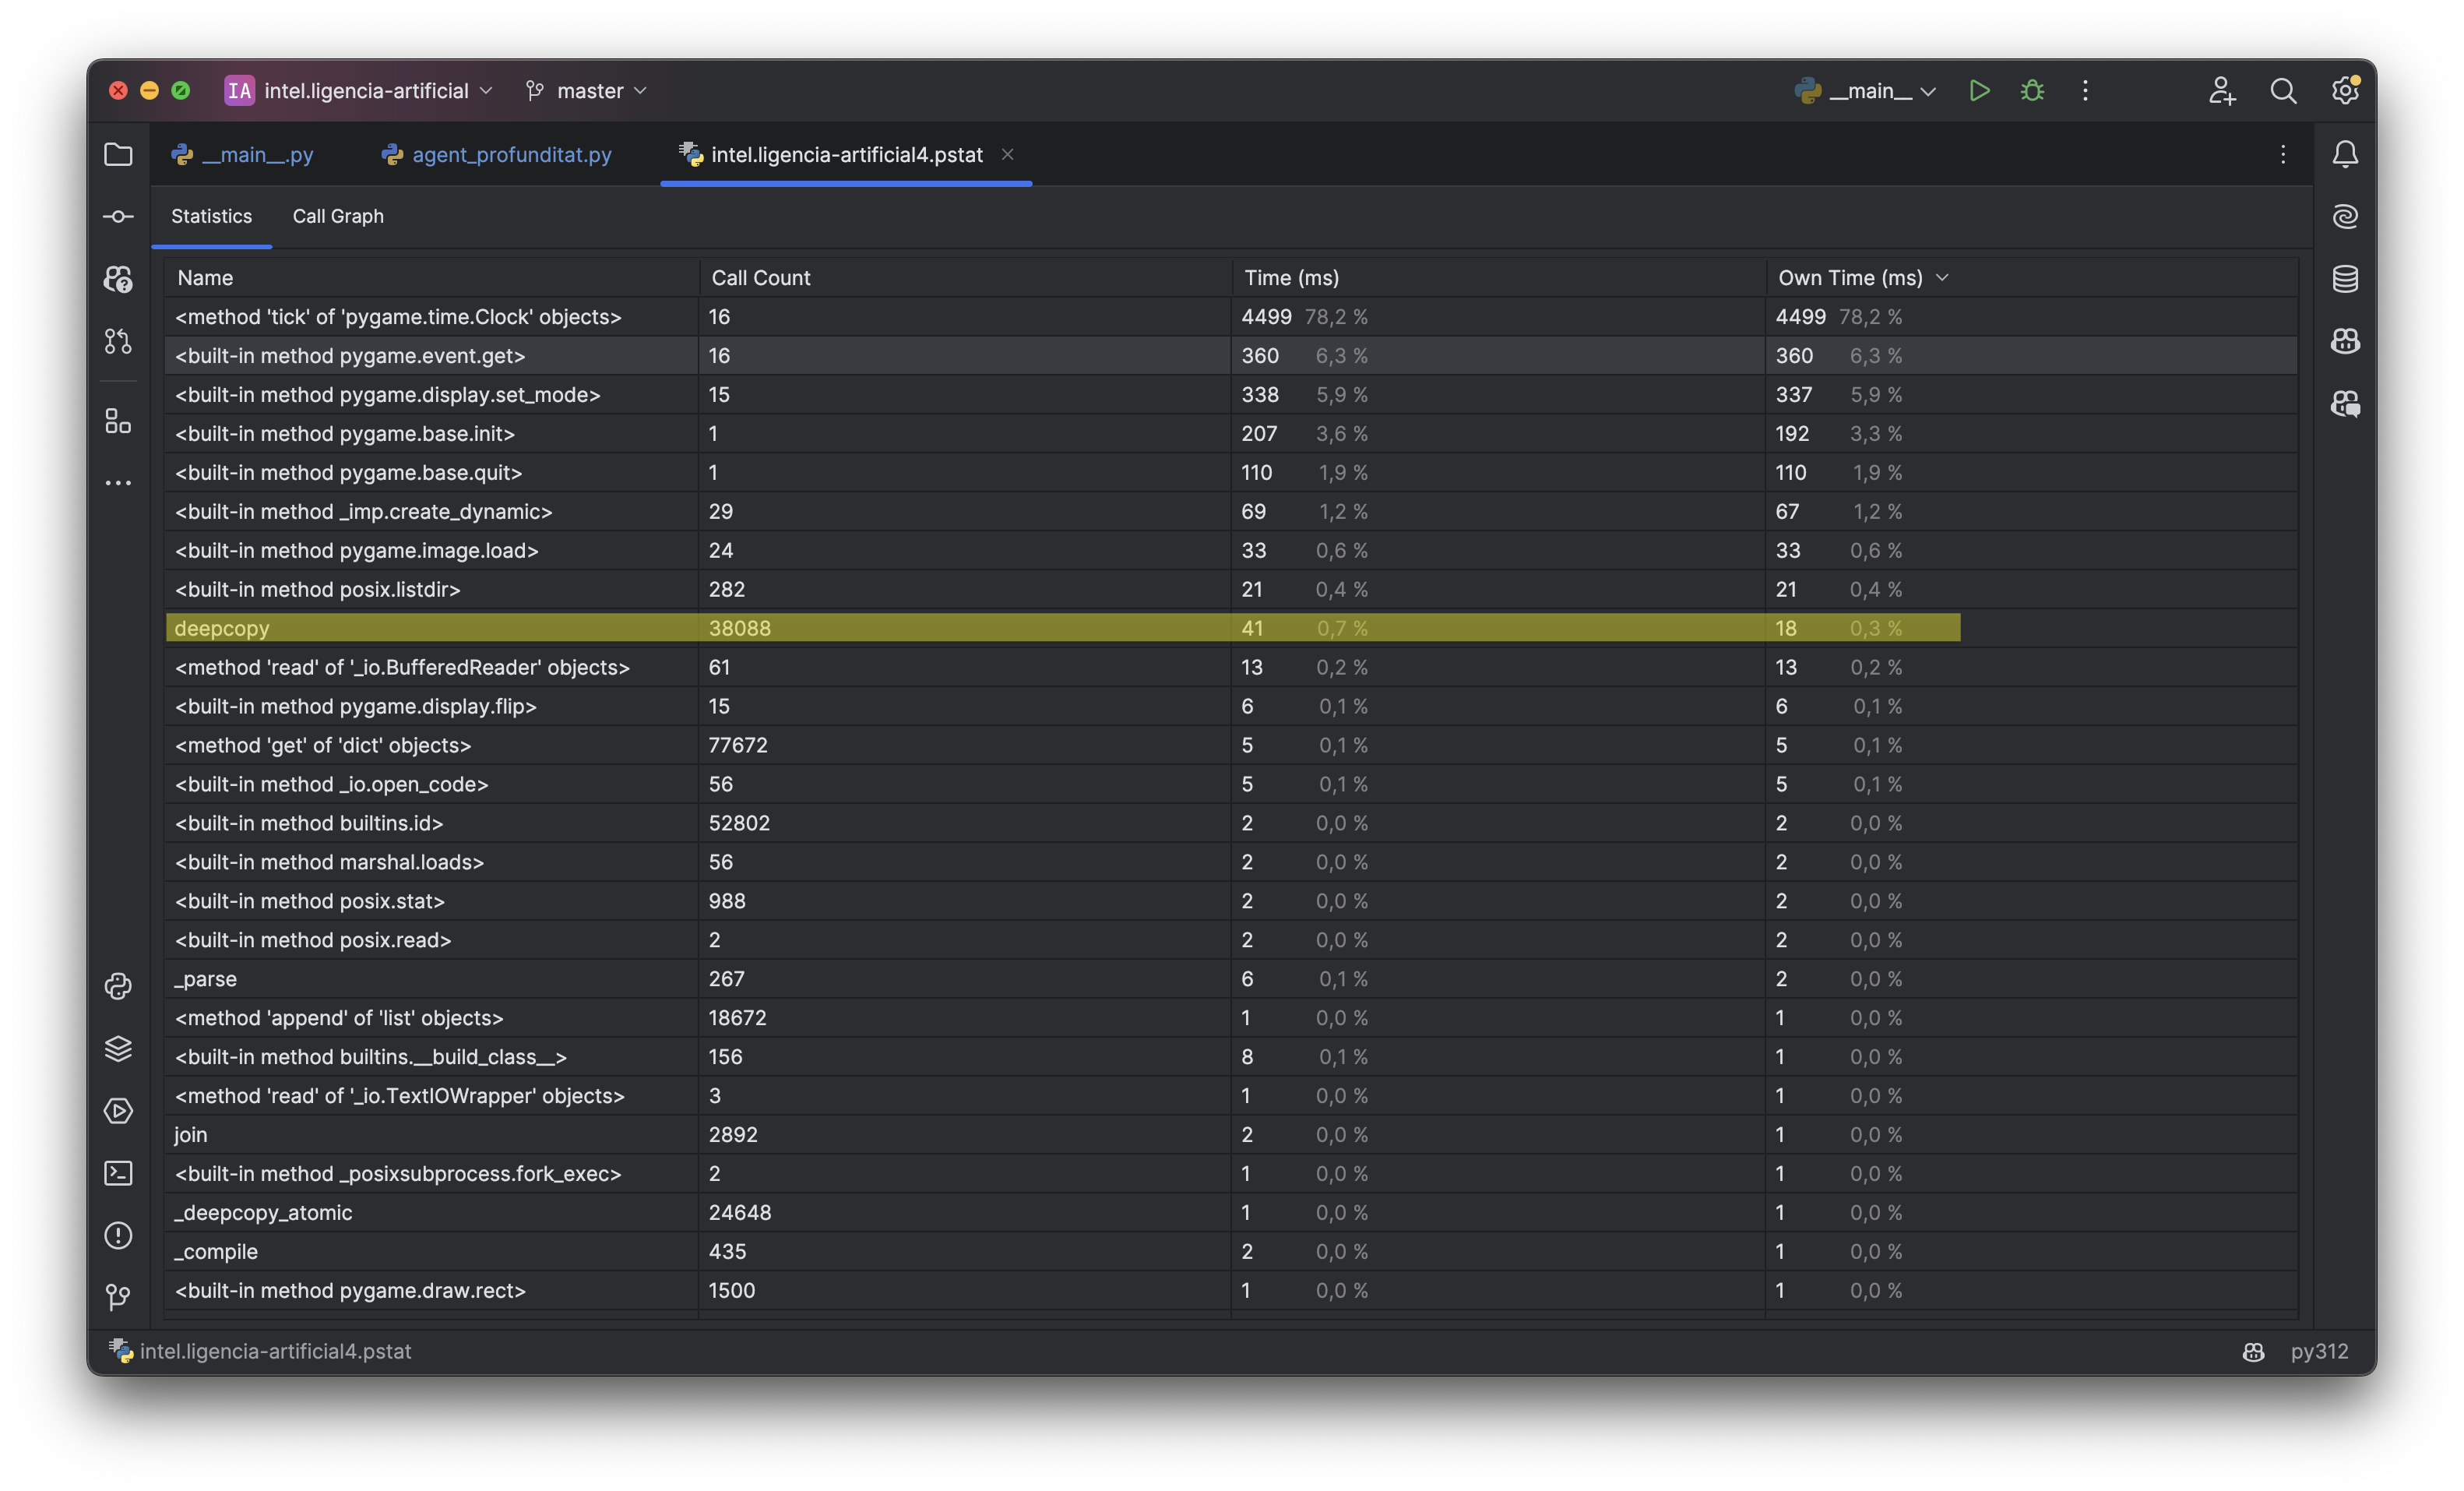
\includegraphics[width=0.72\textwidth]{profunditat.png}
    \caption{Anàlisi amb l'eina \textit{profiling}}
    \label{fig:profunditat-profiling}
\end{figure}

\subsection{\textit{A* Informed Search}}
Els algorismes informats són un canvi de paradigme quasi complet. Aquí apareixen els conceptes d'\href{https://en.wikipedia.org/wiki/Heuristic}{\textit{heurística}} i \textit{cost}. Per a tal de que el nostre agent pugui guiar-se d'alguna forma per tal d'arribar a la casella meta amb una major eficiència, es pot fer ús d'un indicador molt simple: la distància que el separa del seu objectiu. És per això que tenir en compte a l'hora de prendre una decisió sobre el següent moviment la \href{https://en.wikipedia.org/wiki/Taxicab_geometry}{Distància de Manhattan} ens ajuda a assolir l'objectiu més ràpidament. Llavors ara surt la següent qüestió: \textbf{com tenim en compte aquesta distància a l'hora de prendre una decisió?} La resposta a aquesta pregunta es troba dins el mateix algorisme que hem desenvolupat: la fórmula d'A*. 

\subsubsection{La fórmula d'A*}

Aquesta fórmula, similar a la usada en l'algorisme de \href{https://en.wikipedia.org/wiki/Greedy_algorithm}{Greedy} es basa en l'avaluació d'\( f(n) \) definida com:

\[
f(n) = g(n) + h(n)
\]

on:
\begin{itemize}
    \item \( f(n) \) és el \textbf{cost total estimat} d'anar del node \( n \) fins al node destí.
    \item \( g(n) \) és el cost del camí del node inicial al node \( n \).
    \item \( h(n) \) és l'estimació heurística del cost des del node \( n \) fins a la meta.
\end{itemize}

\subsubsection{Codi implementat}
La funció que implementa aquest algorisme és similar a la que hem adjuntat en l'apartat anterior. Encara així, té certs canvis lleus que afecteran considerablement en el rendiment futur. El primer a destacar és l'ús d'una \verb|PriorityQueue| per a gestionar els estats oberts. Com a conseqüència de l'ús d'aquesta estructura de dades, \verb|Python| executa la funció \verb|__lt__| a l'hora d'executar una acció \textit{put}. A aquesta funció \verb|__lt__| (\textit{less than}) li hem fet un \textit{override} perqué inclogui el càlcul de la funció adjunta anteriorment. 

\begin{minted}{python}
def cerca(self, estat_inicial: Estat) -> bool:
  
    self.__oberts = PriorityQueue()
    self.__tancats = set()
    actual = None
    self.__oberts.put(estat_inicial)

    while not self.__oberts.empty():
        actual = self.__oberts.get()
        if actual in self.__tancats:
            continue
        if actual.es_meta():
            self.__accions = actual.accions
            return True
        estats_fills = actual.genera_fills()
        for f in estats_fills:
            self.__oberts.put(f)
        self.__tancats.add(actual)
        
    return False
    
\end{minted}

\newpage

\section{Conclusions}\label{sec:conclusions}
L'ús i aplicació de l’algorisme A* és un salt considerable en l’eficiència i optimalitat de la cerca del nostre agent, coherent amb el que s'espera a l'hora de comparar un algorisme de cerca informada amb un de no-informada. En termes d'estricta eficiència, podem comparar els resultats de la següent taula:
\begin{table}[h]
\centering
$$
\begin{array}{|c|c|c|}
\hline
\text{\textbf{Execució}} & \verb|agent_profunditat.py| & \verb|agent_informat.py| \\
\hline
\text{1} & \text{0,4581 s} & \text{0,0052 s} \\
\text{2} & \text{0,1216 s} & \text{0,0040 s} \\
\text{3} & \text{0,0370 s} & \text{0,0017 s} \\
\text{4} & \text{1,0598 s} & \text{0,0060 s} \\
\text{5} & \text{0,0833 s} & \text{0,0004 s} \\
\text{6} & \text{0,8118 s} & \text{0,0049 s} \\
\text{7} & \text{0,0645 s} & \text{0,0017 s} \\
\text{8} & \text{0,8862 s} & \text{0,0041 s} \\
\text{9} & \text{0,4060 s} & \text{0,0032 s} \\
\hline
\text{\textbf{Mitjana}} & \text{\textit{\textbf{0,4575 s}}} & \text{\textit{\textbf{0,0035 s}}} \\
\hline
\end{array}
$$
\end{table}

Comparant els temps d'execució amb la llibreria \verb|time| hem pogut determinar una mitjana aritmètica del que s'ha trigat després de 9 execucions de cada algorisme. Els resultats són clarament desfavoridors per al primer, doncs es pot veure una reducció de l'ordre de $10^2$. També, una comparativa que hem realitzat és tornar a fer ús del \textit{profiling}, que ens ha marcat un ús de la funció \verb|deepcopy| d'unes \textbf{17256 cridades}, una reducció propera al 50\%. Això és degut a l'implementació d'un algorisme que ens apropa cada pic més a la solució enlloc d'anar explorant l'espai d'estats de forma quasi aleatoria, descartant els nodes que ens allunyen del nostre destí.

Davant l'evidència i claretat que suposen resultats com aquests, és evident que l'aplicació d'algorismes de cerca informada és molt més econòmic que no fer-ho. De totes formes, això només és possible tenint una funció que ens calculi el cost de cada possible decisió que prenem junt amb l'aplicació d'una bona heurística. En aquesta pràctica és molt senzill fer-ho degut a la naturalesa de l'espai d'estats d'aquest "\textit{Grid World}", però determinar una bona heurística que ens sigui útil pot arribar a ser una tasca ben complexa en problemes més avançats.
\end{document}
